%% 参考《控制理论与应用》提供的LATEX模板http://jcta.alljournals.ac.cn/uploadfile/cta_cn/20170419/kzllyy%20template20170419-2.9.zip
%% BHOSC  BUAAthesis  https://github.com/BHOSC/BUAAthesis/
%% 北航学报 http://bhxb.buaa.edu.cn/UserFiles/File/%E5%8C%97%E8%88%AA%E5%AD%A6%E6%8A%A5%E6%A8%A1%E6%9D%BF17.1.16(1).doc

%%%% 五号字对应10.5pt,不知道这样设置对否?
\documentclass[10.5pt,twocolumn]{jbuaa}

%%画圆圈数字
\newcommand*\circled[1]{\tikz[baseline=(char.base)]{
           \node[shape=circle,draw,inner sep=1pt] (char) {#1};}}

%取消英文连词符
% \tolerance=1
% \emergencystretch=\maxdimen
% \hyphenpenalty=10000
% \hbadness=10000

\newcommand\mycolorRed[1]{{\color{red}#1}}
\newcommand\mycolorYellow[1]{{\color{yellow}#1}}
% \newcommand*\mycolorRed{\color{red}}

%%%????? 公式中字体的定义尺寸为 10 磅,上标/下标 68%,次下标/上标 42% ??????
\DeclareMathSizes{10.5}{10}{6.8}{4.2}
%%%% 本示例中带单位的数据采用的是siunitx来生成,好像默认与公式同样大小的字体,所以数字在正文中会小一些
%%%% 行文中普通数字大小为10.5pt,公式里或者用siunitx生成的数字则会是10pt,多少有点不协调。

%%%设置公式前后距离,差不多近似
\setlength{\abovedisplayskip}{2.5mm}
\setlength{\belowdisplayskip}{2.5mm}

\usepackage{tabu}
\usepackage{longtable}
\usepackage{makecell}
\renewcommand\cellgape{\Gape[-3pt][-3pt]}


%%%%%%%%%%%%%%%%%%%%%%%%%%%%%%%%%%%%%%%%%%%%%%%%%%%%%%%%%%%%%%%%
%      文章正文
%%%%%%%%%%%%%%%%%%%%%%%%%%%%%%%%%%%%%%%%%%%%%%%%%%%%%%%%%%%%%%%%
\begin{document}
%%%%%%%%%%%%%%%%%%%%%%%%%%%%%%%%%%%%%%%%%%%%%%%%%%%%%%%%%%%%%%%%
% 标题,基金项目,作者,通信地址定义
%%%%%%%%%%%%%%%%%%%%%%%%%%%%%%%%%%%%%%%%%%%%%%%%%%%%%%%%%%%%%%%%
\title{
\vspace{1cm} \erhao\hei 迁移学习实现猫狗图像分类\vspace{-0.2cm}
}

\author{
\sihao\fang 邓心一,姜百淳,刘姜旺\\[0.1cm]
\liuhao (北京邮电大学~~信息与通信工程学院,北京~~100876)
}

\date{}  % 这一行用来去掉默认的日期显示
%%%%%%%%%%%%%%%%%%%%%%%%%%%%%%%%%%%%%%%%%%%%%%%%%%%%%%%%%%%%%%%%
% 奇数页页眉
%%%%%%%%%%%%%%%%%%%%%%%%%%%%%%%%%%%%%%%%%%%%%%%%%%%%%%%%%%%%%%%%
\fancyhead[CO]{{\footnotesize 迁移学习实现猫狗图像分类}}            %请在这里写出第一作者以及论文题目
%%%%%%%%%%%%%%%%%%%%%%%%%%%%%%%%%%%%%%%%%%%%%%%%%%%%%%%%%%%%%%%%
%%%%%%%%%%%%%%%%%%%%%%%%%%%%%%%%%%%%%%%%%%%%%%%%%%%%%%%%%%%%%%%%
%  显示title,并设页码为空(按杂志社要求)
%%%%%%%%%%%%%%%%%%%%%%%%%%%%%%%%%%%%%%%%%%%%%%%%%%%%%%%%%%%%%%%%
%%%%%%%%%%%%%%%%%%%%%%%%%%%%%%%%%%%%%%%%%%%%%%%%%%%%%%%%%%%%%%%%
%      中文摘要
%%%%%%%%%%%%%%%%%%%%%%%%%%%%%%%%%%%%%%%%%%%%%%%%%%%%%%%%%%%%%%%%
\CKeyword{迁移学习; 图像分类; 卷积神经网络; 模型融合}
\CLCNo{V221\makebox{$^{\scalebox{0.6}{\!+}}$}.3;TB553}
\Dcode{A}
\PaperNo{1001-5965 (XXXX) XX-XXXX-XX}

\twocolumn[
 \begin{@twocolumnfalse}
 \maketitle
\positiontextbox{2.2cm}{2.9cm}{\wuhao http://www.bupt.edu.cn \quad  email@bupt.edu.cn\\[0.3cm]
\wuhao DOI: \ 10.13700/j.bh.1001-5965.****.****}
\begin{CAbstractJBUAA}
本小组选取了kaggle中一道典型的图像分类题目,对数据进行简单预处理,利用迁移学习的思想,采用预训练的卷积神经网络(Convolutional Neural Network, CNN)提取图像的特征向量,使用前馈网络对特征向量进行分类,使用dropout技术防止过拟合,并在Xception模型的基础上引入了InceptionV3和InceptionResNetV2模型,最后采取加权平均的方式进行模型融合,排名能够达到top1\%。在解决问题的过程中,模型经历了多次迭代,数据处理和模型训练也采取了不同的技巧,文章对不同的方法和技巧做出了分析比较,说明了采用迁移学习和模型融合方法的优势。
\end{CAbstractJBUAA}
%%%%%%%%首页角注
\positiontextbox{2.0cm}{25cm}{
\noindent\rule{4cm}{.5pt}\\[0.5ex]%
\hspace*{1em} \liuhao \linespread{0.8}\selectfont
\parbox{\textwidth}{%
\hei\makebox[\widthof{\makebox{*}收}][r]{收}稿日期:2018-01-01; 录用日期:2018-01-01\\%
\hei\makebox[\widthof{\makebox{*}收}][r]{网}络出版地址:(无)\\
\hei\makebox[\widthof{\makebox{*}收}][r]{基}金项目:(无)\\
\hei\makebox[\widthof{\makebox{*}收}][r]{通}信作者:E-mail:\_\_\_@bupt.edu.cn
}}
 \end{@twocolumnfalse}
]


%%%%%%%%%%%%%%%%%%%%%%%%%%%%%%%%%%%%%%%%%%%%%%%%%%%%%%%%%%%%%%%%
%  正文由此开始-------------------------
%%%%%%%%%%%%%%%%%%%%%%%%%%%%%%%%%%%%%%%%%%%%%%%%%%%%%%%%%%%%%%%%
%%%%%%%%%%%%%%%%%%%%%%%%%%%%%%%%%%%%%%%%%%%%%%%%%%%%%%%%%%%%%%%%
\wuhao
%  分栏开始

%%%%%!!!!!正文在第一页两栏分别合适位置插入 \enlargethispage{-3.3cm},给首页跨双栏脚注留空间,大小需要结合前面位置和高度手动设置!!!!!
%%%%%%%%%%%%%%%%%%%%%%%%%%%%%%%%%%%%%%%%%%%%%%%%%%%%%%%%%%%%%%%%
由于卷积神经网络在机器视觉任务中的优秀表现,Kaggle竞赛中与图像相关的题目,绝大多数参赛者采用的是深度学习的解决方案。本小组选择了经典的图像分类任务,在问题的解决过程中,熟悉了一般CNN网络模型的构建方式,尝试运用一些数据挖掘的技巧,提升模型的表现,最终模型分类的准确率令人满意,也在一定程度上减少了模型训练的代价。挖掘任务的详细解决过程陈述如下。

\section{任务描述}
\subsection{竞赛题目}
竞赛题目选用Kaggle竞赛中,类型为Playground的Dogs vs. Cats Redux: Kernels Edition。题目提供已标注的训练集和未标注的测试集,要求参赛者提交测试集中每一张图片为狗的概率。\enlargethispage{-3.3cm}
\begin{equation}
\label{eqnLabel}
Loss=-\frac 1 n\sum_{n}^{i=1}[y_ilog(\hat y_i)+(1-y_i)log(1-\hat y_i)]
\end{equation}
提交的结果用公式(1),即对数损失来衡量。式中,$n$是测试集的图片数量,$\hat y_i$是图片为狗的预测概率,图片实际为猫时,$y_i$取0,否则取1。对数损失越小,预测结果越好。
\subsection{数据集}
数据集分为训练集和测试集,jpg格式。训练集包括12500张猫的图片和12500张狗的图片,大小为543MB,分辨率不等,来自某个宠物领养的网站,推测为程序自动爬取获得,分类标签存在一定程度的错误。测试集包括12500张猫与狗的图片,大小为271MB,来源与训练集相同。

\section{问题定义}
赛题是一个典型的图像分类问题,即根据一定的分类规则将图像自动分到一组预定义类别中。图像分类在多领域有着广泛的实际应用。实际应用中,图像分类任务会受到视角的变化,大小的变化,物体的形变,遮挡,光照条件,\enlargethispage{-3.3cm}背景干扰和多种子类型等各方面因素\citeBUAA{cs231nClassify}的挑战。

对于传统的数据挖掘算法,如K近邻算法(K-Nearest Neighbor, KNN),支持向量机(Support Vector Machine, SVM),图像分类任务是非常复杂甚至难以胜任的。卷积神经网络,以其在图像识别方面的优异表现,从诞生起就备受瞩目。因此,本小组选择CNN作为图像分类算法的核心部分,再利用迁移学习的思想,减少计算量和过拟合的风险。最终将数据挖掘任务划分为以下三个子任务:(1)图像数据的预处理;(2)数据特征的提取;(3)特征处理,对提取出的特征进行分类。

\section{解决方案}
经过多次实验和迭代,本小组最终提出了对图像仅进行简单预处理,以多个卷积神经网络作为特征提取器\citeBUAA{cs231nTransfer},训练前馈神经网络(Feedforward Neural Network, FNN)作为分类器,最后进行模型融合的解决方案。
\subsection{方案提出}
较深的卷积神经网络的训练和计算,需要相当大的计算能力。Google团队2016年提出的Xception模型,使用了60块Nvidia K80 GPUs,在ImageNet数据集上训练了3天\citeBUAA{Xception},达到79\%的Top1准确率。小组最终采用的模型为Inception系列的三个深度均达到100层以上的CNN,而拥有的计算资源仅仅是笔记本上的入门级GPU GTX 1050m,这对计算资源提出了不小的挑战。

此外,虽然相对于小组拥有的计算资源,题目所给训练集数据量较大,但是对于深度神经网络的训练,提供的数据又稍显不足,容易出现过拟合的情况。针对这些问题,在查阅相关资料后,决定采取迁移学习的方式解决。在深度学习的分类器之外,小组也采用了经典的SVM分类器与FNN作出对比。由于采用提取特征向量的方式,需要数据集相对固定,因此难以在短时间内尝试多种数据预处理方式。本小组把模型调整的重心放在网络的后半部分,节约出训练网络的时间来对模型做出优化。因此,形成了简单预处理→CNN提取特征向量→FNN作为分类器→模型融合的方案结构。

以下将从CNN网络、迁移学习和模型融合三个方面来进行算法的介绍。

\subsection{Inception系列网络}
方案选取了在ImageNet数据集中,表现优秀的Inception系列网络,作为特征提取部分的模型。Inception系列网络是Google团队提出的一系列不断改进的CNN模型,名字来源于电影盗梦空间(Inception)中的一句台词:``We need to go deeper''。经典的CNN网络,由负责特征提取的卷积层和负责降采样的池化层交替堆叠而成。Inception系列网络在经典CNN结构的基础上,改进了卷积层的结构,取得了一定的性能提升。

CNN中的卷积核大小,很大程度上影响着提取到的特征图像。一般来说,卷积核越大,感受野越大,越能发现全局的图像特征;卷积核越小,对图像局部的特征更加敏感\citeBUAA{CNNSurvey}。传统的CNN,每一层采用的是一组大小相同的卷积核。为了加强网络的泛化能力,对不同尺度的目标都能良好地识别,InceptionV1提出在同一层采用多种大小的卷积核,将卷积得到的特征向量进行拼接,作为下一层的输入。这就给下一层网络提供了不同尺度上的特征向量信息,使网络能够自由选择,提高了网络的泛化能力。

多个卷积核带来了性能的提升,也带来了极大的计算量。为了减少网络的计算,InceptionV1提出了1×1的卷积核。1×1的卷积核并不会改变特征图像在空间上的相对关系,而是把同一空间位置上的多个通道融合在一起,通过减少输出特征图像的通道数量,达到减少计算量的目的。

为了进一步减少神经网络中的计算,Inception用两个3×3的卷积核代替了一个5×5的卷积核,网络参数由25个下降到18个,还进一步增加了网络的深度。更重要的是,卷积核的感受野是不变的,仍然能够包含5×5的特征图像区域。

此外,1×n和n×1的网络也被引入到Inception网络结构中。

Xecption网络则在另一个角度上对传统CNN的结构作出了改进。区别于传统的卷积核,Xception网络使每一个卷积核仅仅进行一个通道的二位卷积操作,这就将空间上的相关性与通道之间的相关性分离开来。
\subsection{迁移学习}
对于本分类任务而言,由于数据量较大,如果是直接在一个巨大的网络后面加全连接,那么每计算一次前向传播就需要20分钟以上,而且卷积层都是不可训练的,会造成计算资源的浪费,因此我们应用迁移学习(transfer learning)来降低计算开销\citeBUAA{TansferLearning}。下面对这个方法进行一下简单介绍:

迁移学习,顾名思义是把B域中的知识迁移到A域中,以提高A域的分类效果。它作为一种新的学习范式,吸引了众多研究者的注意。对迁移学习的研究来源于一个观测:人类可以将以前的学到的知识应用于处理新的问题,以获得更好的效果。换句话说,迁移学习被赋予这样一个任务:从一个或多个源任务中抽取知识、经验,然后应用到一个新的目标领域当中,从而更快更好地解决问题。

\begin{figure}[h!]
\centering
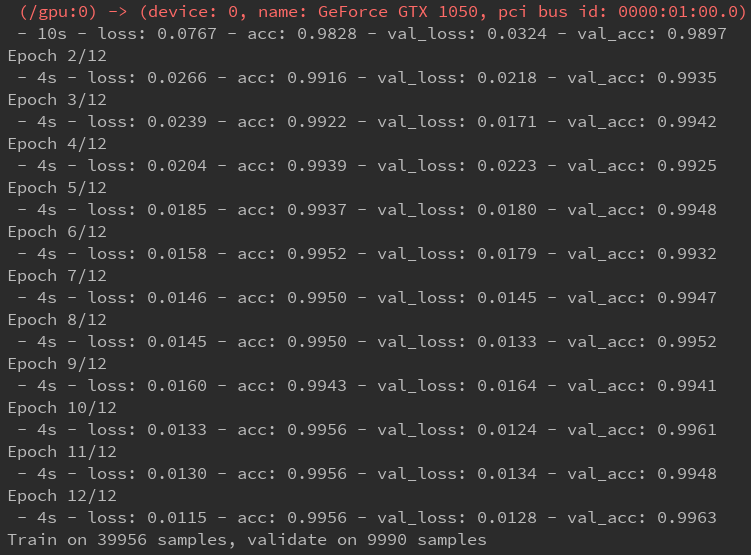
\includegraphics [scale=0.5,trim=0 0 0 0]{./image/training.png}
\bicaption[labelFigtu4]{图}{\centering 训练过程}{Fig.}{\centering training process}
\end{figure}

基于迁移的内容,迁移学习可分为如下几类——基于实例的迁移学习:源领中的数据的某一部分可以通过调整权重的方法重用,用于目标域的学习;基于特征表示的迁移学习:通过源域学习一个好的特征表示,把知识通过特征的形式进行编码,并从源域传递到目标域,提升目标域任务效果;基于参数的迁移学习:目标域和源域的任务之间共享相同的模型参数或者是服从相同的先验分布;基于关系知识的迁移学习:假设源域和目标域中,数据之间联系关系是相同的,从而进行相关领域之间的知识迁移。

\begin{figure}[h!]
\centering
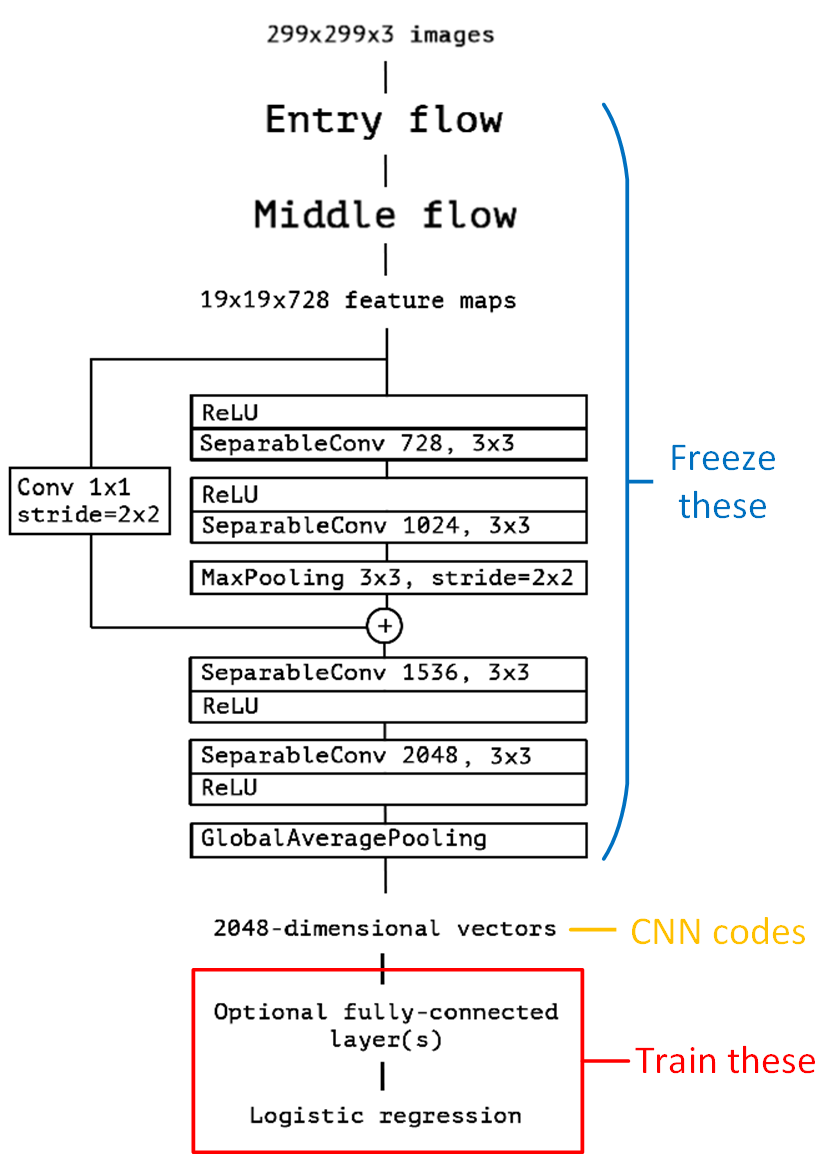
\includegraphics [scale=0.35,trim=0 0 0 0]{./image/xception.png}
\bicaption[labelFigtu5]{图}{\centering 迁移学习示例}{Fig.}{\centering example of transfer learning}
\end{figure}

这之中基于关系知识和参数的迁移学习适用于本项目分类任务,如图\ref{labelFigtu5}具体为固定预训练模型的前半部分网络参数,只训练CNN网络的后半部分,这样无论迭代次数为何,前半部分网络对相同的图像只需经过一次前向传播的计算,大大减少了训练时间。在提取出特征向量之后,仅需要对FNN分类器进行短时间的训练就可以达到良好的训练效果。如图\ref{labelFigtu4}所示,Xception网络提取出的特征向量,仅仅需要54s就能完成12epochs的迭代,并且在验证集上达到了99.63\%的准确率。
\subsection{模型融合}
集成学习(ensemble learning)通过构建并结合多个学习器来完成分类任务,其通过将多个学习器进行结合,常可获得比单一学习器显著优越的泛化性能\citeBUAA{MLBook}。在本项目中,提高模型表现的一种有效方法是综合各个不同的模型(学习器),从而兼听则明,得到更为出色的效果。学习器的结合策略包括平均法、投票法和学习法,本小组采用最常见的平均法来对不同模型的数值型输出进行融合。平均法中的加权平均法(weighted averaging)为:
\begin{equation}
\label{eqnLabel}
H(x)=\sum_{i=1}^{T}\omega_{i}h_{i}(x)
\end{equation}
其中$\omega_{i}$是个体学习器$h_{i}$的权重,通常要求$\omega_{i}\geq0$且$\sum_{i=1}^{T}\omega_{i}=1$。而简单平均法是加权平均法令$\omega_{i}=1/T$的特例。加权平均法在集成学习中具有特别的意义,集成学习中的各种结合方法都可视为其特例或变体:对给定的基学习器,不同的集成学习方法均可等效为通过不同的方式来确定加权平均法中的基学习器权重。这里的权重来自于训练数据,可由正比于各训练模型的准确率或反比于差错率两种方式得到,本小组采用第一种方法来得到各模型的加权权重,实践证明,此种方式取得了较为满意的性能提升。
\begin{figure}[h!]
\centering
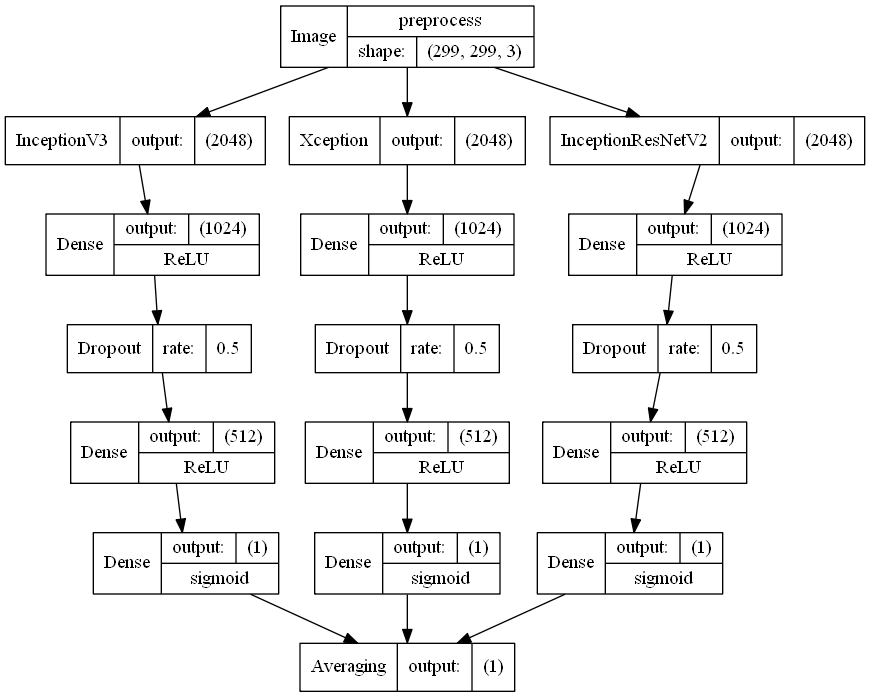
\includegraphics [scale=0.3,trim=0 0 0 0]{./image/final.png}
\bicaption[labelFigtu1]{图}{\centering 最终方案}{Fig.}{\centering final solutuon}
\end{figure}
小组最终采用的模型如图\ref{labelFigtu1}所示。
\section{数据处理}
\subsection{数据预处理}
作为特征提取器的CNN网络需要299×299像素、RGB通道的图像输入。此外,为了加强神经网络的性能,防止过拟合,对图像进行一定程度的数据增强是相当有必要的。为此,需要先对数据做一些预处理工作。

训练集中的图像比例不均,若简单将其拉伸为正方形,则会使物体发生形变。因此需要为图像填充背景后拉伸,以保持图像的比例。背景颜色对图像来说是人为引入的噪声,需要将其影响降到最低。Inception系列网络在输入图像时,会利用公式$x=(x/255-0.5)\times2$对每个像素进行正则化,映射到$[-1,+1]$范围内。因此,将背景色填充为$(127,127,127)$,使其正则化之后最接近0,能在最大程度上减少背景色对数据的影响。

此外,本小组还尝试了几种数据增强的方式:图像翻转,椒盐噪声,直方图均衡。

图像的翻转、旋转是CNN图像处理中最常见的数据增强方式,简单高效,能够有效减少神经网络的过拟合风险。但随着数据量的增大,所需的计算量也随之增加。考虑到现实中(以及测试集中)猫狗图像一般不会有上下颠倒的情况,仅仅采取了水平翻转的方式,实际训练中,在验证集上取得了一定的准确率提升。

\begin{figure}[h!]
\centering
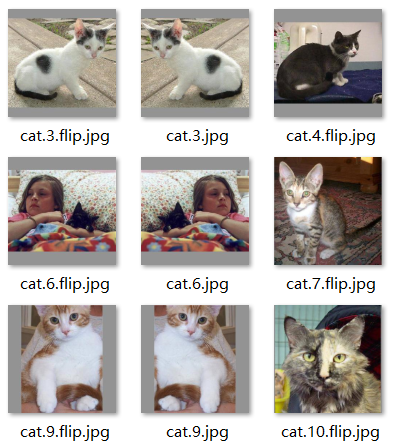
\includegraphics [scale=0.8,trim=0 0 0 0]{./image/preprocess_train.png}
\bicaption[labelFigtu2]{图}{\centering 预处理结果}{Fig.}{\centering result of preprocessing}
\end{figure}

添加椒盐噪声,是指按一定的信噪比随机在图片中添加纯白或纯黑像素点。小组尝试了0.8和0.9的信噪比,发现预测准确率均存在一定程度的下降。推测是椒盐噪声虽然增加了网络的鲁棒性,然而也破坏了图片中携带的信息,使得网络难以辨认图像,从而影响预测的结果。此外,CNN网络是固定不变的,椒盐噪声带来的鲁棒性提升很难被网络所利用。因此,此方案最后并未被采用。

直方图均衡是为了解决部分图像亮度条件较差的问题而采用的方案。它的原理是统计彩色图像中RGB值的累积概率函数,再将其线性化,使得像素点的取值在$[0,255]$之间接近均匀分布,从而增加图像全局的对比度。自适应直方图均衡克服了直方图均衡的缺陷,将图片划分为多个子块,在子块上平衡累积概率分布,从而避免了图像分布被整体移动、背景噪声被加强的缺陷。小组尝试了直方图均衡和自适应直方图均衡两种方式,在实际训练中,并未发现此方法对预测结果有提升。由于预处理之后需要重新进行特征向量的提取,在直方图均衡效果不明显的情况下,将此方案舍弃。

图像随机切割也是一种较好的数据增强方式,考虑随机切割会极大增加数据量,并且极有可能将目标物体排除(一些图片中猫狗的体积非常小),因此并未采用。随机调整对比度、亮度的方案也因为极大地增加了计算量,并未实际采用。
\subsection{特征向量提取}
小组采用在ImageNet数据集中,预训练的InceptionV3,Xception,InceptionResNetV2网络,取最后一层卷积层的输出,经过全局平均池化(即对输出特征图像的每个通道取平均值,三个网络都是2048个通道)后,作为提取出的特征向量。

ImageNet数据集包含至少1000类物体的图像,并且三种Inception网络为了迁移学习的需要,在网络最后一层均保留了1000类的全连接层,所以最后的卷积层得到的特征向量具有良好的泛化能力。网络将同时提取训练集和测试集的特征向量,训练集的特征向量用于训练FNN分类器,测试集的特征向量则用于给出最终的预测结果。

利用本组现有的计算资源,每一个网络提取特征向量的时间平均30分钟,相当于在网络中计算一遍所有图片的前向传播所花费的时间。如果按照通常的训练策略,将所有图片在网络中迭代十次,每个网络,前向传播加上反向传播的时间,可以预计将超过$10\times2\times30=10h$,远远不如单独提取特征向量的运算效率。
\subsection{FNN分类器}
实际使用的FNN分类器是一个两层的前馈神经网络,为了防止过拟合,第一层的输出经过Dropout之后,再输出到第二层网络。理论上,取得特征向量之后,所采用的分类器可以自由选择,为了与FNN做对比,小组采用了传统的SVM分类器进行分类,效果不如FNN。鉴于FNN能够自由调节网络结构,并且在数据量较多时,FNN的分类结果比SVM更为准确\citeBUAA{SVMorFNN},采用FNN作为模型的分类器。

通过迭代次数和网络参数的调节,可以有效地防止FNN出现过拟合,另外,采用验证集,结合early stopping技术,也可以使网络达到局部最优的训练结果。经过多次训练和调试,选择第一层1024个神经元,第二层512个神经元,$50\%$的Dropout比例为参数,$20\%$的数据划分为验证集,为每个网络分别构建FNN分类器,迭代次数根据CNN表达能力的强弱进行了相应调整,梯度下降算法是adam,可以自适应地改变学习率。

\begin{figure}[h!]
\centering
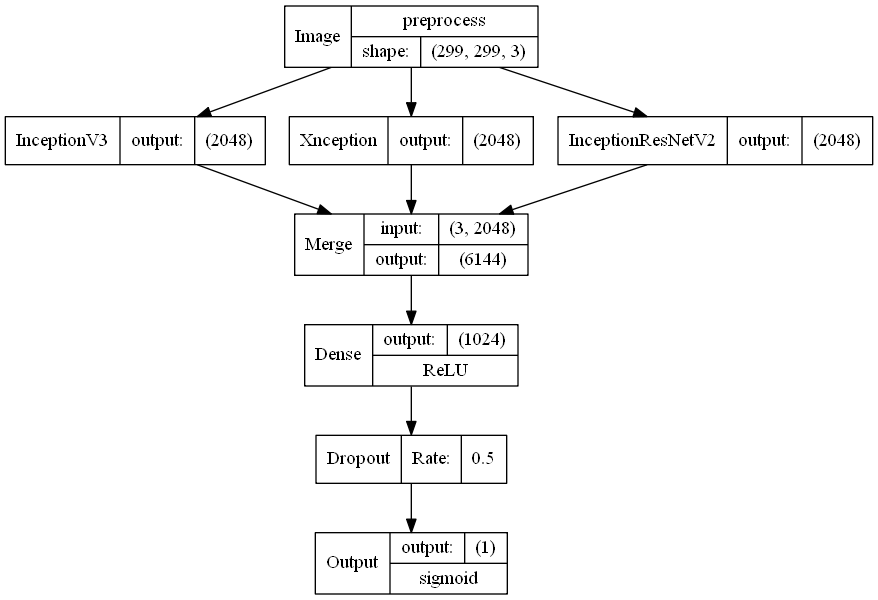
\includegraphics [scale=0.3,trim=0 0 0 0]{./image/concat3.png}
\bicaption[labelFigtu3]{图}{\centering 合并特征向量的方案}{Fig.}{\centering solutuon of combining feature vectors}
\end{figure}

除了为每个网络独立分配FNN分类器之外,如图\ref{labelFigtu3},小组也尝试了将三个网络提取出的特征向量直接拼接,再用同一个FNN分类器进行分类的方案,发现方案的效果不及模型融合,为了得到模型融合的优势,采用了多个分类器的方式。
\subsection{模型融合}
简单起见,小组采用的是加权求平均的方式,将三个网络的预测值,按照其在ImageNet数据集中的Top1准确率进行加权平均。相比仅仅拼接特征向量的方式,模型融合对预测结果有可观的提升。最终网络在本地验证集上的准确率,甚至可以达到$99.8\%$左右(不排除出现了过拟合现象)。

\section{结果分析}
\subsection{预测结果}
表\ref{labelTabtab1}是各个模型预测结果提交后的损失得分和最终排名(由于比赛已经结束,排名参考的是public leaderboard中的LogLoss值)。
\begin{table}[h]
\centering
\captionnamefont{\xiaowuhao\bf }
\captiontitlefont{\xiaowuhao\bf }
\bicaption[labelTabtab1]{表}{预测结果}{Table}{result of prediction}
\renewcommand\tabcolsep{1em}
\begin{tabular}{cccc}
\toprule
{模型} &  {对数损失} & {排名}\\
\midrule
Xception+SVM & 0.05709 & 102\\
Xception+FNN & 0.04475 & 28\\
双模型+FNN & 0.04099 & 18\\
三模型+FNN & 0.03941 & 15\\
最终方案 & 0.03842 & 12\\
\bottomrule
\end{tabular}
\end{table}
分析不同模型之间的差距,可以简单地得到一些结论:

1)SVM与FNN的差距,在于模型所采用的SVM是硬分类器,而FNN是软分类器,因此在分类出错时,SVM受到损失函数的惩罚会更严重;此外,FNN在表达能力和灵活性方面都要优于SVM分类器,样本数量较大时FNN也占优势;

2)表1第三和第四行中采用的模型,是用拼接特征向量的方式组合到一起的,也就是说,每增加一个模型,特征向量的维度都会增加2048,从而获得更全面的特征信息。然而,拼接的特征向量仍然是采用同一个FNN分类器进行训练的,难以回避过拟合的风险;

3)模型加权平均在多模型的基础上为每个CNN特征提取器训练不同的FNN分类器,降低了过拟合的风险,还可以对不同的FNN采取不同的训练策略,小组采用了12epochs、20epochs和12epochs的迭代次数分别对Xception,InceptionV3和InceptionResNetV2进行了训练,弥补了InceptionV3准确率不及另外两个网络的缺陷。
\subsection{误差分析}
CNN在图像识别任务上有出色的表现,但是其运行机理更像是一个黑箱,经过多重网络的乘加等运算,很难定量分析误差的情况。为此,小组从预测结果出发,试图从一个更为直观的角度分析误差产生的原因。

\begin{figure}[h!]
\centering
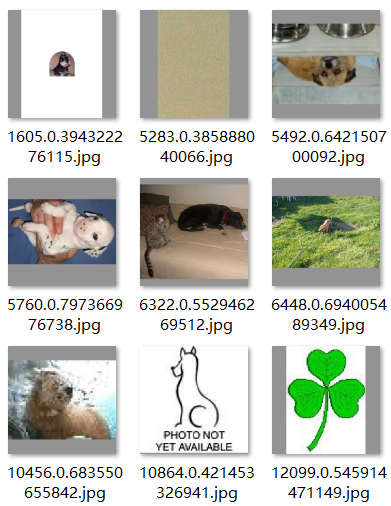
\includegraphics [scale=0.8,trim=0 0 0 0]{./image/low_acc.png}
\bicaption[labelFigtu6]{图}{\centering 准确率较低的预测集图像}{Fig.}{\centering images in test set with low accuracy}
\end{figure}

编写脚本,从预测结果中挑选出概率在$[0.2,0.8]$区间内的图像,部分图像如图\ref{labelFigtu6}所示,共得到134张,通过手工筛查,发现图像有以下特征:

1)错误样本:在训练集和测试集中,均存在无法进行分类的图像,如``Photo Unavailable''、纯色背景、猫狗在同一场景中,非猫狗物体等;2)目标过小:存在目标物体占图像整体比例少于10\%的情况,导致网络难以识别;3)分辨率低:部分测试集图像是由极低分辨率(如$[60,44]$)拉伸而成,与$[299,299]$的网络输入差别较大,无法准确预测;4)部分图片中的猫狗物体有非正常的拍摄角度,如上下倒置,这类角度在训练集中极少出现,导致网络难以预测这部分图片的分类情况。
\subsection{改进方案}
由于时间原因,模型及算法尚有改善空间,具体可在以下几个方面进行优化:

1)使用其他预训练模型(如VGG)进行微调;2)网络调优,可以在已有数据的基础上训练网络的后几个卷积层甚至整个网络;3)使用异常检测\citeBUAA{AnomalyDetection}的方法检测出错误及非常规图像,而后单独标定;4)在得到的特征向量的基础上尝试聚类、随机森林等神经网络之外的数据挖掘方式……这些待完善的地方还会在后续进行探索。

此外,针对误差分析中发现的情况,可以采用相应的数据增强方式(如上下倒置,随机放缩),来提升网络在测试集上的预测效果。

% \vspace{1em}
% {\hei\wuhao 致谢\quad}
% {\fang\wuhao
% }


%%%%%%%%%%%%%%%%%%%%%%%%%%%%%%%%%%%%%%%%%%%%%%%%%%%%%%%%%%%%%%%%
%  参考文献
%%%%%%%%%%%%%%%%%%%%%%%%%%%%%%%%%%%%%%%%%%%%%%%%%%%%%%%%%%%%%%%%
\renewcommand\refname{\hei\wuhao\centerline{参考文献(References)}\global\def\refname{参考文献}}
\vskip 12pt

\let\OLDthebibliography\thebibliography
\renewcommand\thebibliography[1]{
 \OLDthebibliography{#1}
 \setlength{\parskip}{0pt}
 \setlength{\itemsep}{0pt plus 0.3ex}
}

{
\renewcommand{\baselinestretch}{0.9}
\liuhao
\bibliographystyle{unsrt}
\bibliography{./main}
}


%%%%%%%%%%%%%%%%%%%%%%%%%%%%%%%%%%%%%%%%%%%%%%%%%%%%%%%%%%%%%%%%
%  英文摘要页
%%%%%%%%%%%%%%%%%%%%%%%%%%%%%%%%%%%%%%%%%%%%%%%%%%%%%%%%%%%%%%%%
\clearpage
\newpage
% \cleardoublepage
% \cleardoublepage\null
% \newpage\null\thispagestyle{empty}\newpage
\pagestyle{fancy}
\fancyhf{}
\lhead{}
\chead{\vspace{0.8cm}\centering{{\CJKfamily{hei}\xiaowuhao 北\ 京\ 邮\ 电\ 大\ 学}\\[-0.5ex]
{{\xiaowuhao Beijing University of Posts and Telecommunications}}}}
\rhead{}
\lfoot{}
\cfoot{}
\rfoot{}
\renewcommand{\headrule}{%
\hrule height0.4pt width \headwidth \vskip1.0pt%
\hrule height0.4pt width \headwidth \vskip-2pt}


%%%%%%%%%%%%%%%%%%%%%%%%%%%%%%%%%%%%%%%%%%%%%%%%%%%%%%%%%%%%%%%%
%          英文摘要
%%%%%%%%%%%%%%%%%%%%%%%%%%%%%%%%%%%%%%%%%%%%%%%%%%%%%%%%%%%%%%%%
\twocolumn[
\begin{@twocolumnfalse}\vspace*{0.3cm}
\begin{center}
\parbox{\textwidth}{
\setlength{\parindent}{1em}
{
\centering\sihao\textbf{Transfer Learning for Image Classification of Cats and Dogs}\\
} \vspace{-1.2mm}
\begin{center}
{\wuhao DENG Xinyi, JIANG Baichun, LIU Jiangwang}\\[-0.1cm]
\liuhao{(School of Information and Communication Engineering, Beijing University of Posts and Telecommunications, Beijing 100876, China)}
\end{center}

\vspace{-10pt}\wuhao
{
\textbf{Abstract:}
The team selected a typical image classification problem in kaggle, firstly, preprocessing the data , then with the idea of transfer learning, extracted the feature vector of the image using pretrained convolutional neural network. Feedforward neural network is used for classification of the feature vector. What's more, InceptionV3 and InceptionResNetV2 are introduced on the basis of Xception. Finally, the three models are merged by weighted averaging, therefore our ranking can reach top 1\%. Through out the process of problem solving, the model has undergone many iterations, and a variety of methods are applied to data preprocessing. Different methods and techniques have been analyzed and compared, to illustrate the advantages of transfer learning and model ensembling.
\textbf{Key words:} transfer learning; image classification; convolutional neural network; model ensembling
}
}
\end{center}

%%%%%!!!!!英文脚注!!!!!
\positiontextbox{2.0cm}{16cm}{
\noindent\rule{4cm}{.5pt}\\[0.5ex]%
\hspace*{1em} \xiaowuhao \linespread{0.8}\selectfont
\parbox{\textwidth}{%
\CalibriFont
\hei\makebox[\widthof{\makebox{*}\textbf{R}}][r]{\textbf{R}}\textbf{eceived:} 2018-01-01; \textbf{Accepted:} 2018-01-01\\%
\hei\makebox[\widthof{\makebox{*}\textbf{U}}][r]{\textbf{U}}\textbf{RL:} (None)\\
\hei\makebox[\widthof{\makebox{*}\textbf{F}}][r]{\textbf{F}}\textbf{oundation item:} (None)\\
\hei\makebox[\widthof{\makebox{*}\textbf{C}}][r]{\textbf{C}}\textbf{orresponding author.} Tel.: 010-8231xxxx ~~ E-mail: \_\_\_@bupt.edu.cn
}}
 \end{@twocolumnfalse}
]


%%%%%%%%%%%%%%%%%%%%%%%%%%%%%%%%%%%%%%%%%%%%%%%%%%%%%%%%%%%%%%%%
%  英文摘要页 结束
%%%%%%%%%%%%%%%%%%%%%%%%%%%%%%%%%%%%%%%%%%%%%%%%%%%%%%%%%%%%%%%%
\end{document}
